%    2. Write your answers in section "B" below. Precede answers for all 
%       parts of a question with the command "\question{n}{desc}" where n is
%       the question number and "desc" is a short, one-line description of 
%       the problem. There is no need to restate the problem.
%    3. If a question has multiple parts, precede the answer to part x with the
%       command "\part{x}".
%    4. If a problem asks you to design an algorithm, use the commands
%       \algorithm, \correctness, \runtime to precede your discussion of the 
%       description of the algorithm, its correctness, and its running time, respectively.
%    5. You can include graphics by using the command \includegraphics{FILENAME}
%
\documentclass[11pt]{article}
\usepackage{amsmath,amssymb,amsthm}
\usepackage{graphicx}
\usepackage[margin=1in]{geometry}
\usepackage{fancyhdr}
\usepackage{float}
\setlength{\parindent}{0pt}
\setlength{\parskip}{5pt plus 1pt}
\setlength{\headheight}{13.6pt}
\newcommand\question[2]{\vspace{.25in}\hrule\textbf{#1: #2}\vspace{.5em}\hrule\vspace{.10in}}
\renewcommand\part[1]{\vspace{.10in}\textbf{(#1)}}
\pagestyle{fancyplain}
\lhead{\textbf{\NAME\ (\UID)}}
\chead{\textbf{HW\HWNUM}}
\rhead{CS 6390, \today}
\begin{document}\raggedright

\newcommand\NAME{Jake Pitkin}
\newcommand\UID{u0891770}
\newcommand\HWNUM{2}

\question{Problem 1}{Furniture}

\begin{equation}
\setlength\fboxsep{0.25cm}
\setlength\fboxrule{0.4pt}
\boxed{PMI(w_1, w_2) = log_2\bigg(\frac{P(w_1 \ \& \ w_2)}{P(w_1) * P(w_2)}\bigg)}
\end{equation}

\begin{equation}
\setlength\fboxsep{0.25cm}
\setlength\fboxrule{0.4pt}
\boxed{drift(t, n, m) = \frac{AvgSim(L_{1..n}, t)}{AvgSim(L_{(N-m)..N, t})}}
\end{equation}

\part{a} To compute the \textit{semantic drift} score for "futon", first we must compute the point-wise mutual information (PMI) for "futon" and the first 2 words and last 3 words added to the lexicon using eq. 1.

\begin{align*}
&PMI(futon, \ chair) = log_2\bigg(\frac{P(futon, \ chair)}{P(futon) * P(chair)}\bigg) = log_2\bigg(\frac{40}{\frac{60}{2,000} * \frac{200}{2,000}}\bigg) = 13.703 \\
&PMI(futon, \ couch) = log_2\bigg(\frac{P(futon, \ couch)}{P(futon) * P(couch)}\bigg) = log_2\bigg(\frac{20}{\frac{60}{2,000} * \frac{50}{2,000}}\bigg) =  14.703\\
&PMI(futon, \ board) = log_2\bigg(\frac{P(futon, \ board)}{P(futon) * P(board)}\bigg) = log_2\bigg(\frac{50}{\frac{60}{2,000} * \frac{300}{2,000}}\bigg) =  13.44\\
&PMI(futon, \ closet) = log_2\bigg(\frac{P(futon, \ closet)}{P(futon) * P(closet)}\bigg) = log_2\bigg(\frac{25}{\frac{60}{2,000} * \frac{80}{2,000}}\bigg) =  14.347\\
&PMI(futon, \ set) = log_2\bigg(\frac{P(futon, \ set)}{P(futon) * P(set)}\bigg) = log_2\bigg(\frac{60}{\frac{60}{2,000} * \frac{900}{2,000}}\bigg) =  12.118\\
\end{align*}
With the PMI scores, we can calculate the semantic drift using eq. 2.

\begin{align*}
&drift(futon, 2, 3) = \frac{AvgSim([chair, couch], futon)}{AvgSim([board, closet, set], futon)} = \frac{\frac{13.703 + 14.703}{2}}{\frac{13.44 + 14.347 + 12.118}{3}} = \framebox[1.2\width]{1.0678 }\\
\end{align*}

\part{b} We can compute the \textit{semantic drift} score for "hammock" as we did for "futon" is part a. This time we will consider the first 4 words and the last 2 words.

\begin{align*}
&PMI(hammock, \ chair) = log_2\bigg(\frac{P(hammock, \ chair)}{P(hammock) * P(chair)}\bigg) = log_2\bigg(\frac{30}{\frac{10}{2,000} * \frac{200}{2,000}}\bigg) =  15.873\\
&PMI(hammock, \ couch) = log_2\bigg(\frac{P(hammock, \ couch)}{P(hammock) * P(couch)}\bigg) = log_2\bigg(\frac{10}{\frac{10}{2,000} * \frac{50}{2,000}}\bigg) =  16.288\\
&PMI(hammock, \ sofa) = log_2\bigg(\frac{P(hammock, \ sofa)}{P(hammock) * P(sofa)}\bigg) = log_2\bigg(\frac{8}{\frac{10}{2,000} * \frac{40}{2,000}}\bigg) =  16.288\\
&PMI(hammock, \ bed) = log_2\bigg(\frac{P(hammock, \ bed)}{P(hammock) * P(bed)}\bigg) = log_2\bigg(\frac{34}{\frac{10}{2,000} * \frac{100}{2,000}}\bigg) =  17.053\\
&PMI(hammock, \ closet) = log_2\bigg(\frac{P(hammock, \ closet)}{P(hammock) * P(closet)}\bigg) = log_2\bigg(\frac{15}{\frac{10}{2,000} * \frac{80}{2,000}}\bigg) =  16.195\\
&PMI(hammock, \ set) = log_2\bigg(\frac{P(hammock, \ set)}{P(hammock) * P(set)}\bigg) = log_2\bigg(\frac{30}{\frac{10}{2,000} * \frac{900}{2,000}}\bigg) =  13.703\\
\end{align*}

With the PMI scores, we can calculate the semantic drift using eq. 2.

\begin{align*}
drift(futon, 4, 2) &= \frac{AvgSim([chair, couch, sofa, bed], hammock)}{AvgSim([closet, set], hammock)} \\ &= \frac{\frac{15.873 + 16.288 + 16.288 + 17.053}{4}}{\frac{16.195 + 13.703}{2}} = \framebox[1.2\width]{1.0954}\\
\end{align*}

\part{c} I think this similarity metric would be a \textbf{poor choice} for detecting semantic drift. A similarity metric that computes Jaccard distance on a vector of POS statistics would not express the semantic similarity between words in the lexicon and a candidate word.

For example, consider the semantic category FURNITURE we are working with and the 10 initial words in the lexicon. Most of these words would have a POS vector with a very high probability of being a NOUN. Lets take two new candidate words that would also have a very high probability of being a NOUN: \textit{recliner} and \textit{onion}. Both would score a similar semantic drift score under Jaccard distance but \textit{onion} obviously drifts dramatically more than \textit{recliner}.
\question{Problem 2}{Snowball Patterns}

\begin{equation}
\setlength\fboxsep{0.25cm}
\setlength\fboxrule{0.4pt}
\boxed{Match(T_p, T_s) = 
	\begin{cases} 
      	L_p \boldsymbol{\cdot} L_s + M_p \boldsymbol{\cdot} M_s + R_p \boldsymbol{\cdot} R_s & if \ the \ tags \ match \\
      	0 & otherwise \\
	\end{cases}
}
\end{equation}

\part{a} We use eq. 3 to compute the degree of similarity between $P_1$ and $P_2$. The tags match on $P_1$ and $P_2$, so we use case 1 of the piecewise function.

\begin{align*}
Match(P_1, \ P_2) = \ &L_1 \boldsymbol{\cdot} L_2 + M_1 \boldsymbol{\cdot} M_2 + R_1 \boldsymbol{\cdot} R_2  \\ Match(P_1, \ P_2) = \ &((3 * 5) + (4 * 2) + (1 * 2)) + \\ & ((8 * 0) + (9 * 1) + (0 * 9)) + \\ & ((5 * 1) + (0 * 7) + (6 * 4))\\Match(P_1, P_2) = & \ \framebox[1.2\width]{63}
\end{align*}

\part{b} The Tag1 for $P_1$ (LOC) does not match the Tag1 for $P_3$ (PER) so the degree of similarity is zero.

\begin{align*}
Match(P_1, \ P_3) = \framebox[1.2\width]{0}
\end{align*}

\part{c} Similar to part a, we use case 1 of the piecewise function.

\begin{align*}
Match(P_1, \ P_4) = \ &L_1 \boldsymbol{\cdot} L_4 + M_1 \boldsymbol{\cdot} M_4 + R_1 \boldsymbol{\cdot} R_4  \\ Match(P_1, \ P_4) = \ &((3 * 0) + (4 * 9) + (1 * 5)) + \\ & ((8 * 3) + (9 * 2) + (0 * 6)) + \\ & ((5 * 4) + (0 * 2) + (6 * 1))\\Match(P_1, P_4) = & \ \framebox[1.2\width]{109}
\end{align*}

\question{Problem 3}{Hypernyms}

\part{a}

\begin{figure}[H]
  \centerline{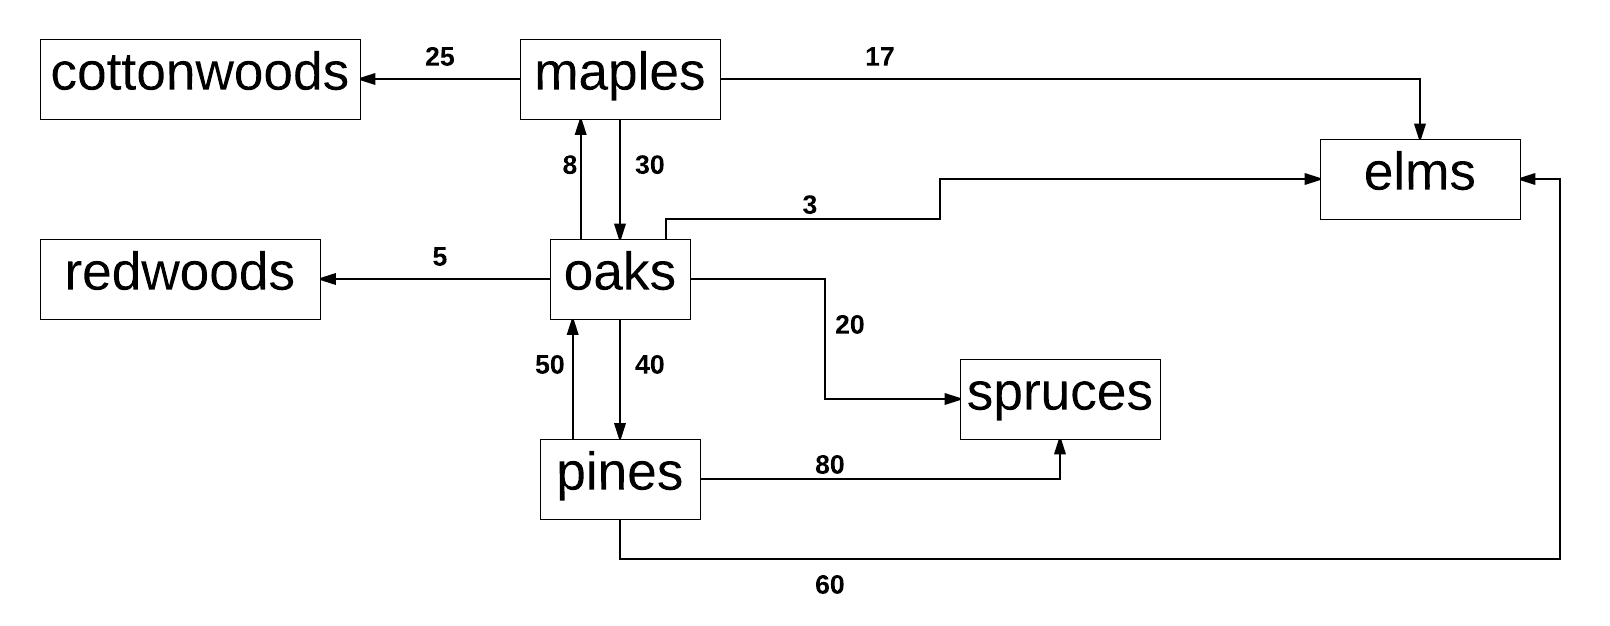
\includegraphics[width=0.5\linewidth]{hplg.png}}
  \caption{HPLG representing the web query table.}
\end{figure}

\part{b} The function $weight(u, v)$ returns the weight of a directed edge from node $u$ to node $v$. If such an edge doesn't exist, 0 is returned.

\begin{align*}
Popularity(pines) &= \sum_{v \in V}^{|V|} weight(v, pines) \\
&= weight(oaks, pines) \\
&= \framebox[1.2\width]{40} \\ \\
Popularity(oaks) &= \sum_{v \in V}^{|V|} weight(v, oaks) \\
&= weight(maples, oaks) + weight(pines, oaks) \\
&= 30 + 50 \\
&= \framebox[1.2\width]{80} \\ \\
Popularity(spruces) &= \sum_{v \in V}^{|V|} weight(v, spruces) \\
&= weight(oaks, spruces) + weight(pines, spruces) \\
&= 20 + 80 \\
&= \framebox[1.2\width]{100}
\end{align*}

\part{c} 

\begin{align*}
Productivity(pines) &= \sum_{v \in V}^{|V|} weight(pines, v) \\
&= weight(pines, oaks) + weight(pines, spruces) + weight(pines, elms) \\
&= 50 + 80 + 60 \\
&= \framebox[1.2\width]{190}	 \\ \\
\end{align*}
\begin{align*}
Productivity(oaks) = &\sum_{v \in V}^{|V|} weight(oaks, v) \\
= &weight(oaks, maples) + weight(oaks, pines) + \\ &weight(oaks, elms) + weight(oaks, spruces) + weight(oaks, redwoods) \\
= &8 + 40 + 3 + 20 + 5\\
= &\framebox[1.2\width]{76} \\ \\
Productivity(spruces) &= \sum_{v \in V}^{|V|} weight(spruces, v) \\
&= \framebox[1.5\width]{0}
\end{align*}

\part{d} The Concept Positioning Test (CPT) is used to determine if a learned hypernym is more general than our Root Concept "plants". Given the two patterns:
\vskip 0.2in
\centerline{\textbf{(a)} $<$Hypernym$>$ such as plants and *}
\vskip 0.1in
\centerline{\textbf{(b)} plants such as $<$Hypernym$>$ and *}
\vskip 0.2in
We will consider a learned hypernym to be less general than "plants" and pass the test if the following are true:

\vskip 0.2in
\centerline{Pattern (b) produces at least 50 hits.}
\vskip 0.1in
\centerline{Pattern (b) returns at least 4 times as many hits as pattern (a).}
\vskip 0.2in

\part{d.i} \textit{ferns}: \textbf{would} - Ferns are a hyponym of plants so I would expect the pattern \textit{plants such as ferns and *} to produce at least 50 hits and to appear much more often than \textit{ferns such as plants and *} which sounds unnatural.

\part{d.ii} \textit{things}: \textbf{would not} - I expect the pattern \textit{plants such as things and *} to produce little to no hits as things are not a hyponym of plants. Additionally, \textit{things such as plants and *} would produce substantially more hits as plants are a hyponym of things.

\part{d.iii} \textit{vegetables}: \textbf{would not} - I don't expect the pattern \textit{plants such as vegetables and *} to yield many hits. The word vegetables is most commonly used to describe parts of a plant for consumption and sound unnatural in this pattern. Additionally, in biology the word vegetables is used to describe all plant matter so in this context it would not be a hyponym of plants.

\part{d.iv} \textit{succulents}: \textbf{would} - Similar to ferns, succulents are a hyponym of plants so the phrase \textit{plants such as succulents and *} sounds natural and would be common.

\part{d.v} \textit{organisms}: \textbf{would not} - The root concept plants in a hyponym of organisms. Because of this I expect the test to fail as the phrase \textit{plants such as organisms and *} is nonsense.

\question{Problem 4}{Identifying Monetary Amounts}

\part{a} $P(O \ | \ E)$: \textbf{CAN} - This feature represents the probability of moving from state $E$ to state $O$. This would be an entry in the transition probability matrix. This is a legal state transition as \textit{other} could follow the \textit{end} of a named entity.

\part{b} $P(IsNumber(w_i) \ | \ C)$: \textbf{CANNOT} - HMM's are a local generative model and cannot use arbitrary features. We would have to use a MEMM to use a richer feature such as this. 

\part{c} $P(w_i \ | \ O)$: \textbf{CAN} - This is the state observation likelihood of the observation symbol $w_i$ given the current state is $O$.

\part{d} $P(B \ | \ IsCapitalized(w_i))$: \textbf{CANNOT} - This is neither a transition probability or an emission probability and not allowed in the HMM model.

\part{e} $P(C \ | \ C)$: \textbf{CAN} - Represents the probability of moving from state $C$ to state $C$ and is an entry in the transition probability matrix. This would also be a legal state transition as \textit{continue} would follow \textit{continue} in a named entity that is at least four words long.

\part{f} $ContainsDollarSign(w_i)$: \textbf{CANNOT} - HMM's are a local generative model and cannot use global features such as this one. We could use a model such as a CRF or structured perceptron.

\part{g} $P(w_i \ | \ U)$: \textbf{CAN} - The state observation likelihood of the observation symbol $w_i$ given the current state is $U$.

\end{document}